\documentclass[hidelinks,12pt]{article}

\usepackage[brazil]{babel}
\usepackage[utf8]{inputenc}
\usepackage{amsmath}
\usepackage{amsfonts}
\usepackage{amssymb}
\usepackage{indentfirst}
\usepackage{color}
\usepackage{mathrsfs}
\usepackage{pgfplots}
\usepackage{hyperref}
\usepackage{fancyhdr}
\usepackage{graphicx}
\usepackage[export]{adjustbox}
\newcommand{\icon}[1]{\includegraphics[height=12pt]{#1}}
\newcommand{\bigicon}[1]{\includegraphics[height=50pt]{#1}}

\newcommand{\iconb}[1]{\includegraphics[height=20pt]{#1}}
\setcounter{secnumdepth}{5}

\fancypagestyle{plain}{%
	\fancyfoot{}%
	\fancyhead{}%
}


\begin{document}
\pagenumbering{gobble}
\pagestyle{fancy}


\lhead{\bigicon{Figures/ufu}}
\chead{{\footnotesize UNIVERSIDADE FEDERAL DE UBERLÂNDIA \\ FACULDADE DE CIÊNCIA DA COMPUTAÇÃO \\ Inteligência Computacional} \\ \scriptsize{Av. João Naves de Ávila 2121, Campus Santa Mônica} }
\rhead{\bigicon{Figures/facom}}
\lfoot{}
\cfoot{}
\rfoot{}
\vspace*{10cm}
\begin{figure}[!h]
	\centering
	\Huge{Redes Neurais aplicadas ao reconhecimento de matrizes}
\end{figure}


\newpage
\fancyhead[C]{}
\fancyhead[R]{}
\fancyhead[L]{\leftmark}
\fancyfoot{}
\fancyfoot[L]{{\footnotesize  Inteligência Computacional}}
\fancyfoot[C]{\hspace{1.5cm}\thepage}
\fancyfoot[R]{{\footnotesize Redes Neurais}}
\pagenumbering{arabic}


\tableofcontents

{\let\thefootnote\relax\footnotetext{\textit{UFU, Universidade Federal de Uberlândia, Minas Gerais, Brasil}}}

\newpage

\section{Introdução}

	O relatório informa as resoluções dos exercícios pedidos no trabalho de redes neurais, bem como as abordagens utilizadas para chegar às respostas desejadas.

\section{Especificação}
	
	
	\subsection{Representação das matrizes}
	
		As matrizes estão representadas em arquivos de 0 ou 1. São seis linhas e cinco colunas em um \emph{.txt} . 
		\begin{table}[!h]
			\centering
			\begin{tabular}{lllll}
				0 & 0 & 1 & 0 & 0 \\
				0 & 1 & 1 & 0 & 0 \\
				0 & 0 & 1 & 0 & 0 \\
				0 & 0 & 1 & 0 & 0 \\
				0 & 0 & 1 & 0 & 0 \\
				1 & 1 & 1 & 1 & 1
			\end{tabular}
		\end{table}
		
	\subsection{Representação dos pesos}
		
		Os pesos serão representados na forma de matriz sendo que o primeiro peso estará deslocado, possuindo uma linha somente para ele. Esse peso é referente ao bias.
		
\section{Exercícios}

	Seguem as respostas para os exercícios 1, 2 e 3 referentes ao trabalho.
	
	
	\subsection{Exercício 1}
		
		\textbf{\large Com o vetor de pesos zerado inicialmente}
		
		\subsubsection{Vetor de Pesos}
		\begin{figure}[!h]
			\centering
			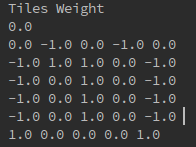
\includegraphics[scale=0.7]{Figures/E1F1.png}
		\end{figure}
		
		\subsubsection{Número de épocas para se aprender um padrão}
		
		Foram necessárias três épocas para atingir o vetor de pesos acima.
		
		\subsubsection{Saída da rede para entradas distorcidas de 0 e 1}
		
		Para as entradas distorcidas. Obteve-se 100\% de eficácia.
		
		Em virtude de testar a rede neural com exemplos mais drásticos, foi inserida uma matriz de 1 tendo como resultado esperado o 0. A rede neural errou dizendo que o valor correto era 1. Segue o exemplo:
		
		\begin{figure}[!h]
			\centering
			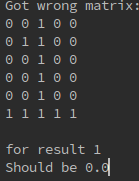
\includegraphics[scale=0.7]{Figures/E1F2.png}
		\end{figure}
		
		\subsubsection{Saída da rede para as entradas de números 2, 3, 4, 5}
		
		A rede neural respondeu que a matriz de número 2 correspondia ao número 1 e as demais matrizes (3, 4, 5) correspondiam ao número 0.\\
		
		\textbf{\large Com o vetor de pesos aleatório entre valores de -1 a 1}
		
		\subsubsection{Vetor de Pesos}
		
		\begin{figure}[!h]
			\centering
			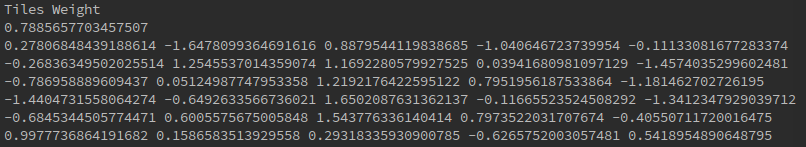
\includegraphics[scale=0.5]{Figures/E1F3.png}
		\end{figure}
		
		\subsubsection{Número de épocas para se aprender um padrão}
		
		Foram necessárias, em média, duas épocas para atingir o vetor de pesos acima.
		
		\subsubsection{Saída da rede para entradas distorcidas de 0 e 1}
		
		Para as entradas distorcidas. Obteve-se 95\% de eficácia. A rede neural errou a seguinte entrada.
		
		\begin{figure}[!h]
			\centering
			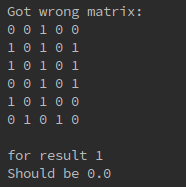
\includegraphics[scale=0.7]{Figures/E1F4.png}
		\end{figure}
		
		Interpreta-se como admissível o erro dado à proximidade que a matriz possui com o 1.	
	
		O exemplo de mandar uma matriz 1 como sendo 0 obteve o mesmo resultado neste esquema de peso.
		
		\subsubsection{Saída da rede para as entradas de números 2, 3, 4, 5}
		
		A rede neural respondeu que a matriz de número 2 correspondia ao número 1 e as demais matrizes (3, 4, 5) correspondiam ao número 0.
	
	

	\subsection{Exercício 2}
	
		A rede entende a saída (1,0) como sendo correspondente ao número 1 e a saída (0,1) correspondente ao 0. As demais saídas representam que a rede não foi capaz de dizer se a matriz era 1 ou 0.\\
		
		\textbf{\large Com o vetor de pesos zerado inicialmente}
		\subsubsection{Vetores de Peso}
		
		\begin{figure}[!h]
			\centering
			
		\begin{tabular}{ll}
			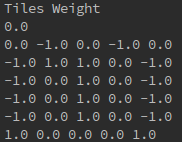
\includegraphics[scale=0.7]{Figures/E2F1.png}
			&
			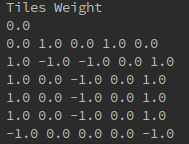
\includegraphics[scale=0.7]{Figures/E2F2.png}
		\end{tabular}
			
		\end{figure}
		
		\subsubsection{Número de épocas para se aprender um padrão}
			
			Foram necessárias 2 épocas para um neurônio e 3 para o outro.
		
		\subsubsection{Saída da rede para entradas distorcidas de 0 e 1}
		
			Para as entradas distorcidas. Obteve-se 100\% de eficácia.
			O exemplo de mandar uma matriz 1 como sendo 0 obteve o mesmo resultado neste esquema de peso.
		
		\subsubsection{Saída da rede para as entradas de números 2, 3, 4, 5}
		
			A rede neural respondeu que a matriz de número 2 correspondia ao número 1 e as demais matrizes (3, 4, 5) correspondiam ao número 0.\\
			
		\newpage
		\textbf{\large Com o vetor de pesos aleatório entre valores de -1 a 1}
		\subsubsection{Vetor de Pesos}
			
		\begin{figure}[!h]
			\centering
			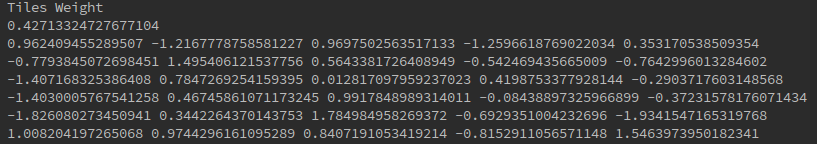
\includegraphics[scale=0.5]{Figures/E2F3.png}
		\end{figure}
		
		\begin{figure}[!h]
			\centering
			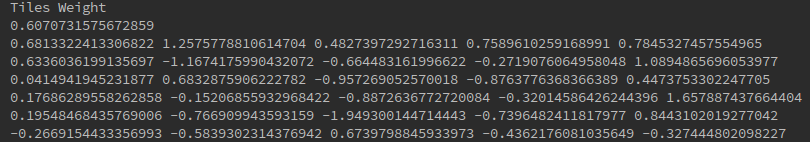
\includegraphics[scale=0.5]{Figures/E2F4.png}
		\end{figure}
			
		\subsubsection{Número de épocas para se aprender um padrão}
			
			Em média, duas épocas para cada um dos dois neurônios.
			
		\subsubsection{Saída da rede para entradas distorcidas de 0 e 1}
		
		Obteve-se uma eficácia de 80\%, sendo que a rede neural não errou nenhuma matriz. Ela respondeu que não sabia identificar o padrão.
		O exemplo de mandar uma matriz 1 como sendo 0 obteve o mesmo resultado neste esquema de peso.
		
		\subsubsection{Saída da rede para as entradas de números 2, 3, 4, 5}
		
		A rede neural respondeu que a matriz de número 2 correspondia ao número 1 e a matriz 3 à 0. Para as entradas 4 e 5, a rede neural não soube responder (a saída dos neurônios foram 1 e 1).
		
	\subsection{Exercício 3}
		
		\textbf{\large Com o vetor de pesos zerado inicialmente}
		
		\subsubsection{Vetor de Pesos}
			
		\begin{figure}[!h]
			\centering
			
			\begin{tabular}{lll}
				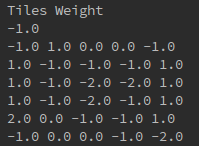
\includegraphics[scale=0.7]{Figures/E3F1.png}
				&
				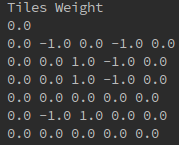
\includegraphics[scale=0.7]{Figures/E3F2.png}
			\end{tabular}
			
			\begin{tabular}{lll}
				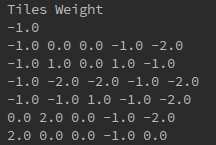
\includegraphics[scale=0.7]{Figures/E3F3.png}
				&
				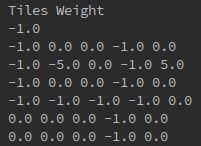
\includegraphics[scale=0.7]{Figures/E3F4.png}
			\end{tabular}
			
			\begin{tabular}{lll}
				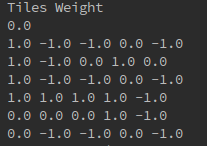
\includegraphics[scale=0.7]{Figures/E3F5.png}
				&
				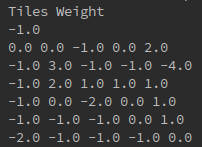
\includegraphics[scale=0.7]{Figures/E3F6.png}
			\end{tabular}
			
		\end{figure}
		
		\subsubsection{Número de épocas para se aprender um padrão}
			
			As épocas necessárias para que os neurônios aprendessem o padrão são 3, 2, 3, 6, 2 e 6 respectivamente. Em torno de 3.6 épocas por neurônio.
			
		\subsubsection{Saída da rede para entradas distorcidas de 0 e 1}
		
			Percebe-se que as amostras alteram de forma significativa o desempenho da rede. Dadas as amostras de testes feitas pelo aluno, o desempenho da rede foi de 68\%.
		
		\subsubsection{Saída da rede para as entradas de letras C, E, H, N, T}
		
			Para as letras C e E, não foi encontrado um padrão (a rede respondeu 00000).
			
			Para H foi respondido 000010, ou seja, 4.
			
			Para N e T foi respondido 010000, ou seja, 1.\\
		
		\textbf{\large Com o vetor de pesos aleatório entre valores de -1 a 1}
		
		\subsubsection{Vetor de Pesos}
		
			\begin{figure}[!h]
				\centering
				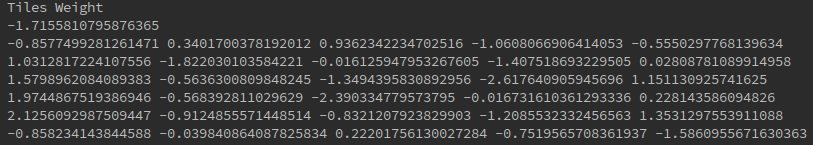
\includegraphics[scale=0.5]{Figures/E3F7.png}
			\end{figure}
			\begin{figure}[!h]
				\centering
				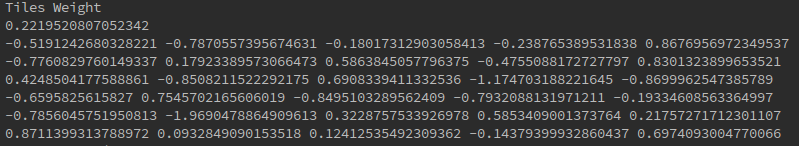
\includegraphics[scale=0.5]{Figures/E3F8.png}
			\end{figure}
			\begin{figure}[!h]
				\centering
				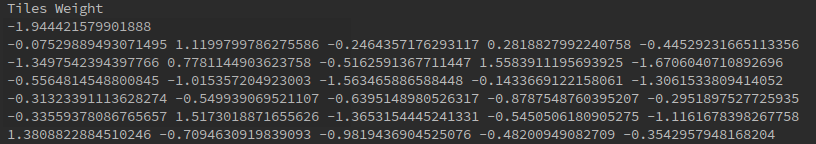
\includegraphics[scale=0.5]{Figures/E3F9.png}
			\end{figure}
			\begin{figure}[!h]
				\centering
				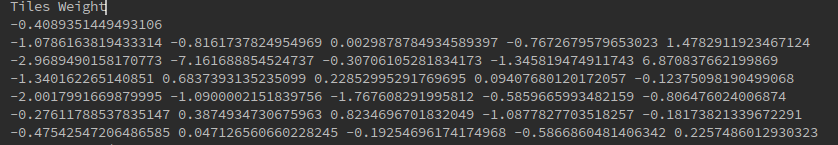
\includegraphics[scale=0.5]{Figures/E3F10.png}
			\end{figure}
			\begin{figure}[!h]
				\centering
				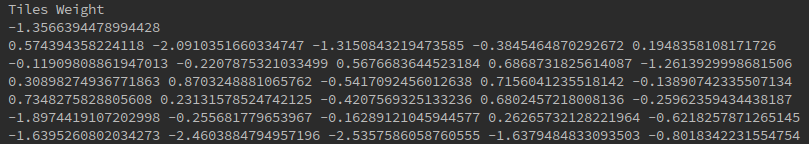
\includegraphics[scale=0.5]{Figures/E3F11.png}
			\end{figure}
			\begin{figure}[!h]
				\centering
				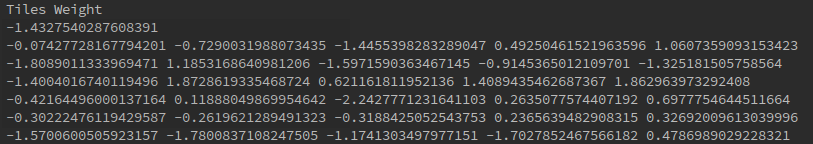
\includegraphics[scale=0.5]{Figures/E3F12.png}
			\end{figure}
			
		\newpage
		\subsubsection{Número de épocas para se aprender um padrão}
			
			As épocas necessárias para que os neurônios aprendessem o padrão são, na média 4, 2, 4, 7, 3 e 4 respectivamente. Em torno de 4.8 épocas de treinamento por neurônio.
			
		\subsubsection{Saída da rede para entradas distorcidas de 0 e 1}
		
			A eficiência da rede depende muito do vetor de pesos. Como eles são iniciados aleatóriamente, é de se esperar que a eficácia possua uma grande margem de erro que está entre 55\% e 70\%.
		
		\subsubsection{Saída da rede para as entradas de letras C, E, H, N, T}
		
			Os resultados variam completamente em detrimento do esquema de pesos adotado pela rede. No exemplo dado, a rede respondeu que o C e E correspondiam ao 1 e para as demais letras não foi obtida resposta alguma. Ao executar o programa múltiplas vezes percebeu-se que:
			
			\begin{itemize}
				\item \textbf{C}: rede não sabe responder;
				\item \textbf{E}: respostas variam entre não reconhecido e raramente 0 e 4;
				\item \textbf{H}: respostas variam entre não reconhecido, 0 e 4;
				\item \textbf{N}: respostas variam entre não reconhecido, 1 e 4. Raramente 2;
				\item \textbf{T}: respostas variam entre não reconhecido e 1.
			\end{itemize} 
	
\end{document}